\documentclass[border = 1.5cm]{standalone}

    %%%% packages
\usepackage{tikz}
\usetikzlibrary{trees,
                arrows,
                shapes.geometric,
                positioning,
                calc,
                backgrounds,
                fit}
%% document
\begin{document}
%% layers
\pgfdeclarelayer{bg1}    % declare background layer
\pgfdeclarelayer{bg2}
\pgfdeclarelayer{bg3}
\pgfsetlayers{bg3, bg2, bg1, main}  % set the order of the layers (main is the standard layer)
%% styles
\tikzset{
	font = {\fontsize{13pt}{12}\sffamily},
	children/.style = {anchor = west},
	ecotox/.style = {rectangle, minimum width = 4cm, minimum height = 3cm, text centered, draw = black, fill = blue!10},
	data/.style = {rectangle, minimum width = 7cm, minimum height = 3cm, text centered, rounded corners, draw = black},
	app/.style = {circle, minimum height = 3cm, text centered, fill = red!40},
	api/.style = {circle, minimum height = 3cm, text centered, fill = red!40},
	rpackage/.style = {circle, minimum height = 3cm, text centered, fill = red!40},
	ids/.style = {diamond, minimum width = 3cm, minimum height = 2cm, text centered, draw = black, fill = green!30},
	db/.style = {rectangle, text centered, draw = black, rounded corners, minimum width = 3cm, minimum height = 1.25cm},
	arrow1/.style = {->, > = stealth, draw = black, color = gray!80, line width = 2.5pt},
	arrow2/.style = {->, > = latex, draw = black, line width = 10pt},
	arrow3/.style = {draw = gray!10, line width = 2cm},
	background/.style = {rectangle, rounded corners, draw = black, fill=gray!0.01}
}

\begin{tikzpicture}
%% nodes
% pipeline
\node (epa-ecotox) [ecotox, above of = epa-ecotox-clean, yshift = 5cm] {EPA};
\node (epa-ecotox-clean) [ecotox, align = center] at (-3cm,0cm) {EPA ECOTOX\\data base\\(cleaned)};
\node (cas) [ids, below of = epa-ecotox-clean, xshift = 6cm, yshift = 3cm] {CAS};
\node (taxa) [ids, below of = cas, xshift = 0cm, yshift = -2.5cm] {Taxa};
\node (db-chemical) [db, right of = cas, xshift = 4cm, align = center] {Chemical\\data bases};
\node (db-habitat) [db, right of = taxa, xshift = 4cm, yshift = 1cm, align = center] {Habitat\\data bases};
\node (db-region) [db, right of = taxa, xshift = 4cm, yshift = -1cm, align = center] {Region\\data bases};
% standartox data
\node (stx-data) [ecotox, below of = epa-ecotox-clean, xshift = 7.5cm, yshift = -6.4cm, align = center] {Standartox\\data set};
% user interfaces
\node (stx-app) [app, below of = stx-data, yshift = -5cm, xshift = -2cm, align = center] {Web\\application};
\begin{pgfonlayer}{bg1}
    \node (stx-app-screenshot) [below of = stx-app, xshift = -2cm] {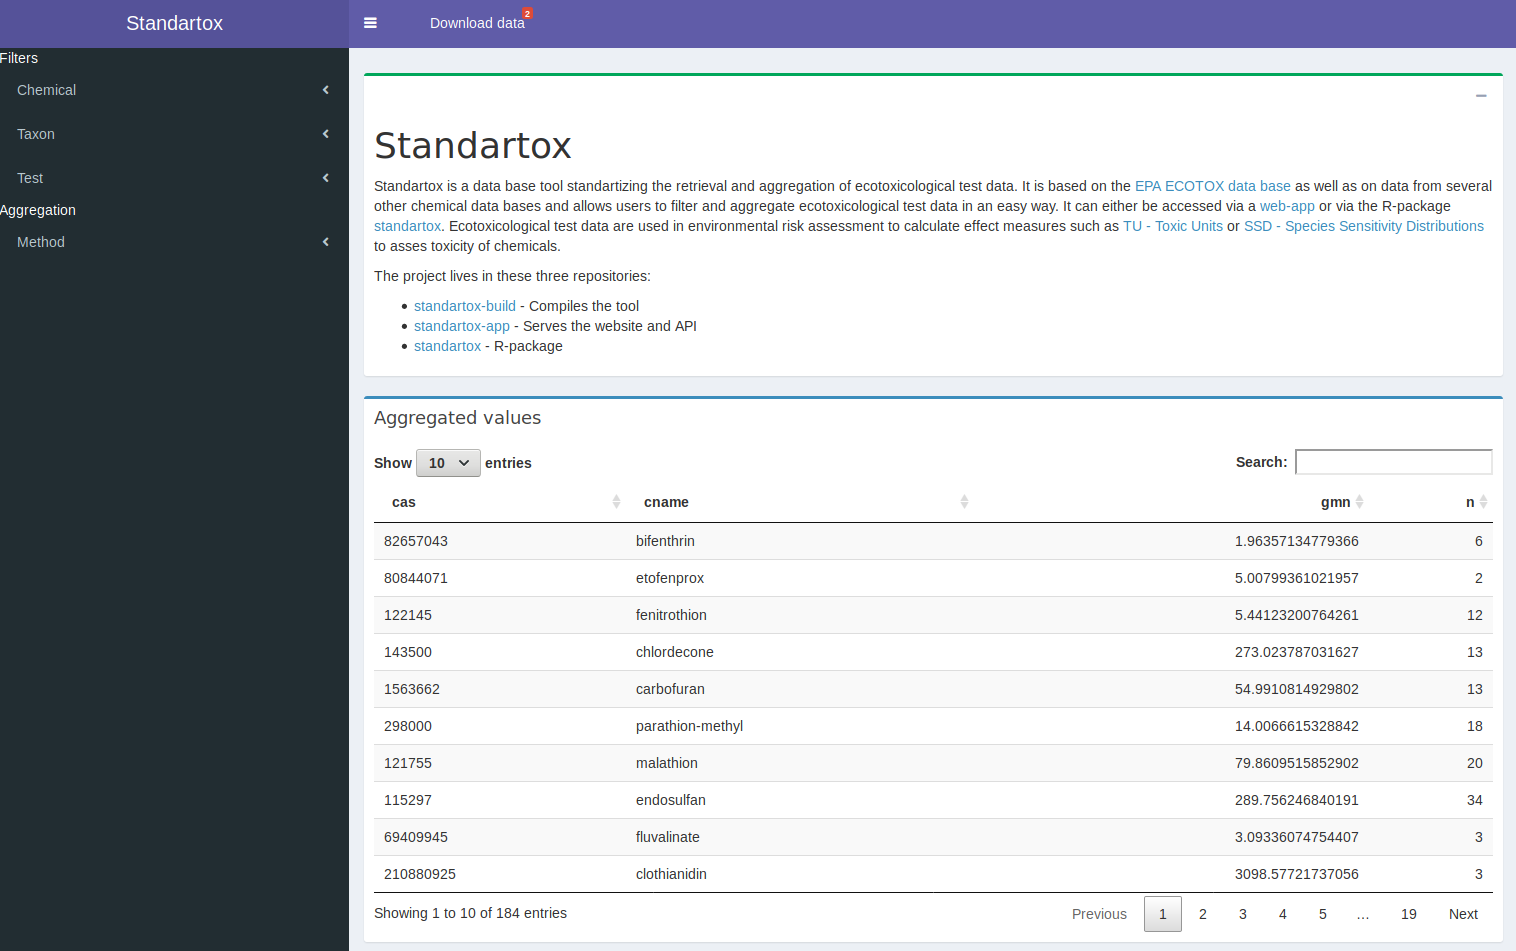
\includegraphics[width=.5\textwidth]{article/figures/screenshot_standartox_app.png}};
\end{pgfonlayer}
\node (stx-api) [api, below of = stx-data, yshift = -5cm, xshift = 2cm] {API};
\node (stx-rpackage) [rpackage, below of = stx-api, yshift = -2cm, xshift = 2cm] {R-package};
\begin{pgfonlayer}{bg1}
    \node (stx-rpackage-screenshot) [below of = stx-rpackage] {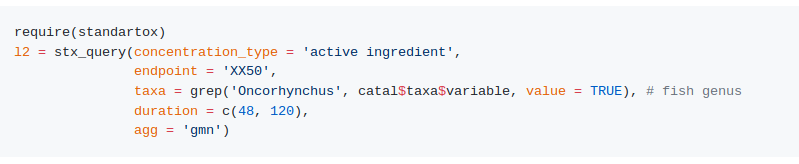
\includegraphics[width=.7\textwidth]{article/figures/screenshot_standartox_rpackage.png}};
\end{pgfonlayer}
%% backgrounds
\begin{pgfonlayer}{bg2}
    %\node (bg1-pipeline) [background, minimum height = 9cm, minimum width = 17cm, above of = epa-ecotox-clean, xshift = 5.5cm, yshift = -1cm];
    % \node (bg1-user) [background, below of = bg1-pipeline, minimum height = 8cm, minimum width = 17cm, yshift = -13cm, xshift = 5cm];
    \draw [arrow3] (12cm,0cm) arc[radius = 7.5cm, start angle = 0, delta angle = 360];
\end{pgfonlayer}
%% arrows
% small
\draw [arrow1] (epa-ecotox-clean.east) -- (cas.west);
\draw [arrow1] (epa-ecotox-clean.east) -- (taxa.west);
\draw [arrow1] (cas.east)-- (db-chemical.west);
\draw [arrow1] (taxa.east) -- (db-habitat.west);
\draw [arrow1] (taxa.east) -- (db-region.west);
\begin{pgfonlayer}{bg2}
    \draw [->, > = latex, draw = gray!10, line width = 1cm] (stx-data.south) -- node[auto] ++ (0cm,-4cm);
\end{pgfonlayer}
\draw [arrow1] (stx-api) -- (stx-rpackage);

\end{tikzpicture}
\end{document}